\section{Phá vỡ chắt lọc phòng thủ}
Ngoài ra, để tấn công DNN không phòng thủ bằng các mẫu đối nghịch, tác giả đã cho thấy EAD có thể phá vỡ DNN chắt lọc phòng thủ. Chắt lọc phòng thủ (Papernot et al. 2016b) là kĩ thuật phòng thủ chuẩn trong đó mạng được huấn luyện lại bằng các xác xuất từng lớp được dự đoán bởi một mạng gốc (chứ không phải bằng nhãn ground truth), gọi là nhãn mềm và người ta dùng tham số nhiệt $T$ trong lớp softmax để tăng cường sức mạnh của nó chống lại nhiễu đối nghịch. Tương tự như phương thức tấn công tiên tiến C\&W, hình \ref{fig:fg_03} cho thấy EAD có thể thu được ASR $100\%$ với các giá trị $T$ khác nhau trên tập MNIST và CIFAR10. Hơn nữa, vì công thức tấn công C\&W là trường hợp đặc biệt của công thức EAD trong (\ref{eq:7}) khi $\beta = 0$, sự thành công của EAD trong việc phá vỡ chắt lọc phòng thủ gợi ý 1 cách mới để tạo ra các mẫu đối nghịch hiệu quả là dùng các tham số  $\beta$ khác nhau cho hiệu chỉnh $L_1$. Kết quả đầy đủ của tấn công ở trong tài liệu mở rộng.

\begin{figure}[H] % places figure environment here   
    \centering % Centers Graphic
    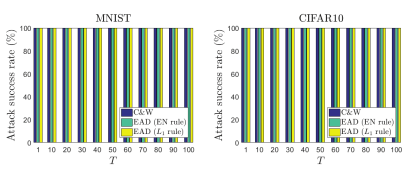
\includegraphics[width=0.8\textwidth]{assets/fig_3.png} 
    \caption{ASR (trường hợp trung bình) của C\&W và EAD trên tập MNIST và CIFAR10 với các tham số nhiệt $T$ khác nhau cho chắt lọc phòng thủ. Cả 2 phương pháp đều phá vỡ thành công chắt lọc phòng thủ.} % Creates caption  % Creates caption underneath graph
    \label{fig:fg_03}
\end{figure}